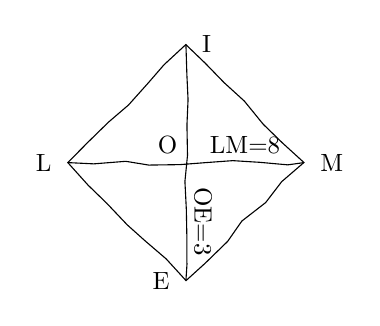
\begin{tikzpicture}[rotate=0,every node/.style={scale=0.9},scale=1]

\coordinate (L) at (0,0);
\coordinate (I) at (1.5,1.5);
\coordinate (M) at (3,0);
\coordinate (E) at (1.5,-1.5);
\coordinate (O) at (1.5,0); %le centre du losange

\draw[decorate,decoration={random steps,amplitude=1pt,segment length=10pt}] (L) node [left=3pt]{L}--(I) node [right=3pt]{I} --(M) node [right=3pt] {M}--(E) node [left=3pt] {E}--cycle;
\draw [decorate,decoration={random steps,amplitude=1pt,segment length=10pt}] (L)--(M) (I)--(E);
\node at (O)[above left]{O}; 
\path (O)--(E) node[midway,above,sloped]{OE=3};
\path (O)--(M) node[midway,above]{LM=8};
\end{tikzpicture}
